\documentclass[a4paper, 10pt]{article}

%\usepackage{cmap}
\usepackage[T2A]{fontenc}
\usepackage[utf8]{inputenc}
\usepackage[english, russian]{babel}
\usepackage{graphicx}
\usepackage[top=2cm, bottom=2cm, left=3cm, right=2cm]{geometry}
\graphicspath{./}
\usepackage{biblatex}
\addbibresource{lib.bib}
\linespread{1.5}
{\usefont{T2A}{Tempora-TLF}{m}{n}
\usepackage{amsmath}

\usepackage{ragged2e}
\justifying

\usepackage{listings}
\usepackage{color}

\makeatletter
\renewcommand{\fnum@figure}{Рисунок \thefigure}
\makeatother

\usepackage{caption}
\captionsetup{labelsep=endash}


\begin{document}
	
\begin{titlepage}
	\fontsize{12pt}{12pt}\selectfont
	\begin{figure}[t!]
		\centering
		
\includegraphics[scale=0.8]{bmstu}
	\end{figure}
	
	\noindent\rule{15cm}{3pt}
	\newline\newline
	\noindent 
	ФАКУЛЬТЕТ 
	\underline{«Информатика и системы управления»} \newline
	
	\noindent КАФЕДРА \underline{«Программное обеспечение ЭВМ и информационные технологии»}\newline\newline\newline
	
	\centering {\Large \textbf{\hspace*{1cm}ОТЧЕТ ПО ПРОИЗВОДСТВЕННОЙ ПРАКТИКЕ}}\newline 
	\begin{flushleft}
		Студент:\hspace{10mm}$\underset{\text{(Фамилия, имя, отчетсво)}}{\underline{\hspace{3cm}\text{Турсунов Жасурбек Рустамович}\hspace{3cm}}}$
	\end{flushleft}

	\begin{flushleft}
		Группа:\hspace{12mm}${\underline{\hspace{5.2cm}\text{ИУ7-66Б}\hspace{5.3cm}}}$
	\end{flushleft}

	\begin{flushleft}
		Тип практики:\hspace{12mm}${\underline{\hspace{3.2cm}\text{производственная	}\hspace{4.2cm}}}$
	\end{flushleft}

	\begin{flushleft}
		Название предприятия:\hspace{5mm}${\underline{\hspace{3cm}\text{ООО <<ПолисСофт>>}\hspace{3.2cm}}}$
	\end{flushleft}

	\vspace*{2cm}


	\begin{flushleft}
		Студент
		\hspace{57mm}$\underset{\text{(Подипсь, дата)}}{\underline{\hspace{40mm}}}$ 
		\hspace{4mm}$\underset{\text{(И.О.Фамилия)}}{\underline{\hspace{2mm}\text{Ж.Р.Турсунов}\hspace{2mm}}}$ 
	\end{flushleft}
	
	\begin{flushleft}
		Руководитель практики
		\hspace{27mm}$\underset{\text{(Подипсь, дата)}}{\underline{\hspace{4cm}}}$ 
		\hspace{4mm}$\underset{\text{(И.О.Фамилия)}}{\underline{\hspace{1mm}\text{Н.Б.Толпинская}\hspace{1mm}}}$ 
	\end{flushleft} 
	
	\begin{flushleft}
		Руководитель предприятия
		\hspace{2cm}$\underset{\text{(Подипсь, дата)}}{\underline{\hspace{4cm}}}$ 
		\hspace{4mm}$\underset{\text{(И.О.Фамилия)}}{\underline{\hspace{3mm}\text{Д.Е.Бекасов}\hspace{6mm}}}$ 
	\end{flushleft} 

	\vspace*{1cm}
	\begin{flushleft}
		Оценка:\underline{\hspace{3cm}}
	\end{flushleft}   
	
	\begin{center}
		\vfill
		Москва, \the\year
		~г.
	\end{center}
	
\end{titlepage}
\setcounter{page}{3}
\tableofcontents
\clearpage
\newpage


\section*{Введение}
\addcontentsline{toc}{section}{Введение}

%\begin{flushleft}
	\hspace*{5mm}Картинг приобретает все большую популярность и как развлечение, и как вид спорта. Во многих городах появляются картодромы, где можно получить дозу адреналина, улучшить свои навыки вождения, снять стресс и просто весело провести время. Спортивный картинг является основой гоночного вида спорта. И как для любого пилота, периодически нужно выполнять анализ пройденного маршрута, для улучшения навыков вождения. Для получения такого анализа достаточно подключить необходимые приборы к карту и специальное программное обеспечение поможет сделать вывод о пройденном мрашруте.
	 
	\vspace{1cm}\hspace*{-5mm}\textbf{Цель данной работы} - разработка программно-аппаратного комплекса для оценки качества прохождения маршрутов.
	 \vspace{1cm}\\\textbf{Задачи проекта:}
	 \begin{enumerate}
	 	\item построение траектории пройденного маршрута;
	 	\item оценка качества прохождения маршрута пилотом;
	 	\item визуализация полученной оценки.
	 \end{enumerate}
	 \textbf{Индивидуальные задачи:}
	 \begin{enumerate}
	 	\item получить навыки командной разработки;
	 	\item разобраться уже в существующей реализации сервиса и в используемых технологиях;
	 	\item написать документацию к новым функциям для API;
	 	\item добавить новые функции в API;
	 	\item провести модульное тестирование;
	 	\item провести нагрузочное тестирование и сделать анализ полученных результатов.
	 \end{enumerate}
%\end{flushleft}
\clearpage
\newpage
\section*{Основная часть}
\addcontentsline{toc}{section}{Основная часть}
%\begin{flushleft}
	\section{Декомпозиция функциональной части}
	На рисунке 1 показан нулевой уровень функциональной модели IDEF0 для разрабатываемого программного-аппаратного комплекса, а на рисунке 2 подробно описан первый уровень данной модели. Для проведения оценки качества прохождения маршрута нужно знать маршрут трека и маршрут который был пройден фактически картом. В качестве выходных данных должна выступать визуализация оценки качества прохождения маршрута.
	\begin{figure}[h!]
		\centering
		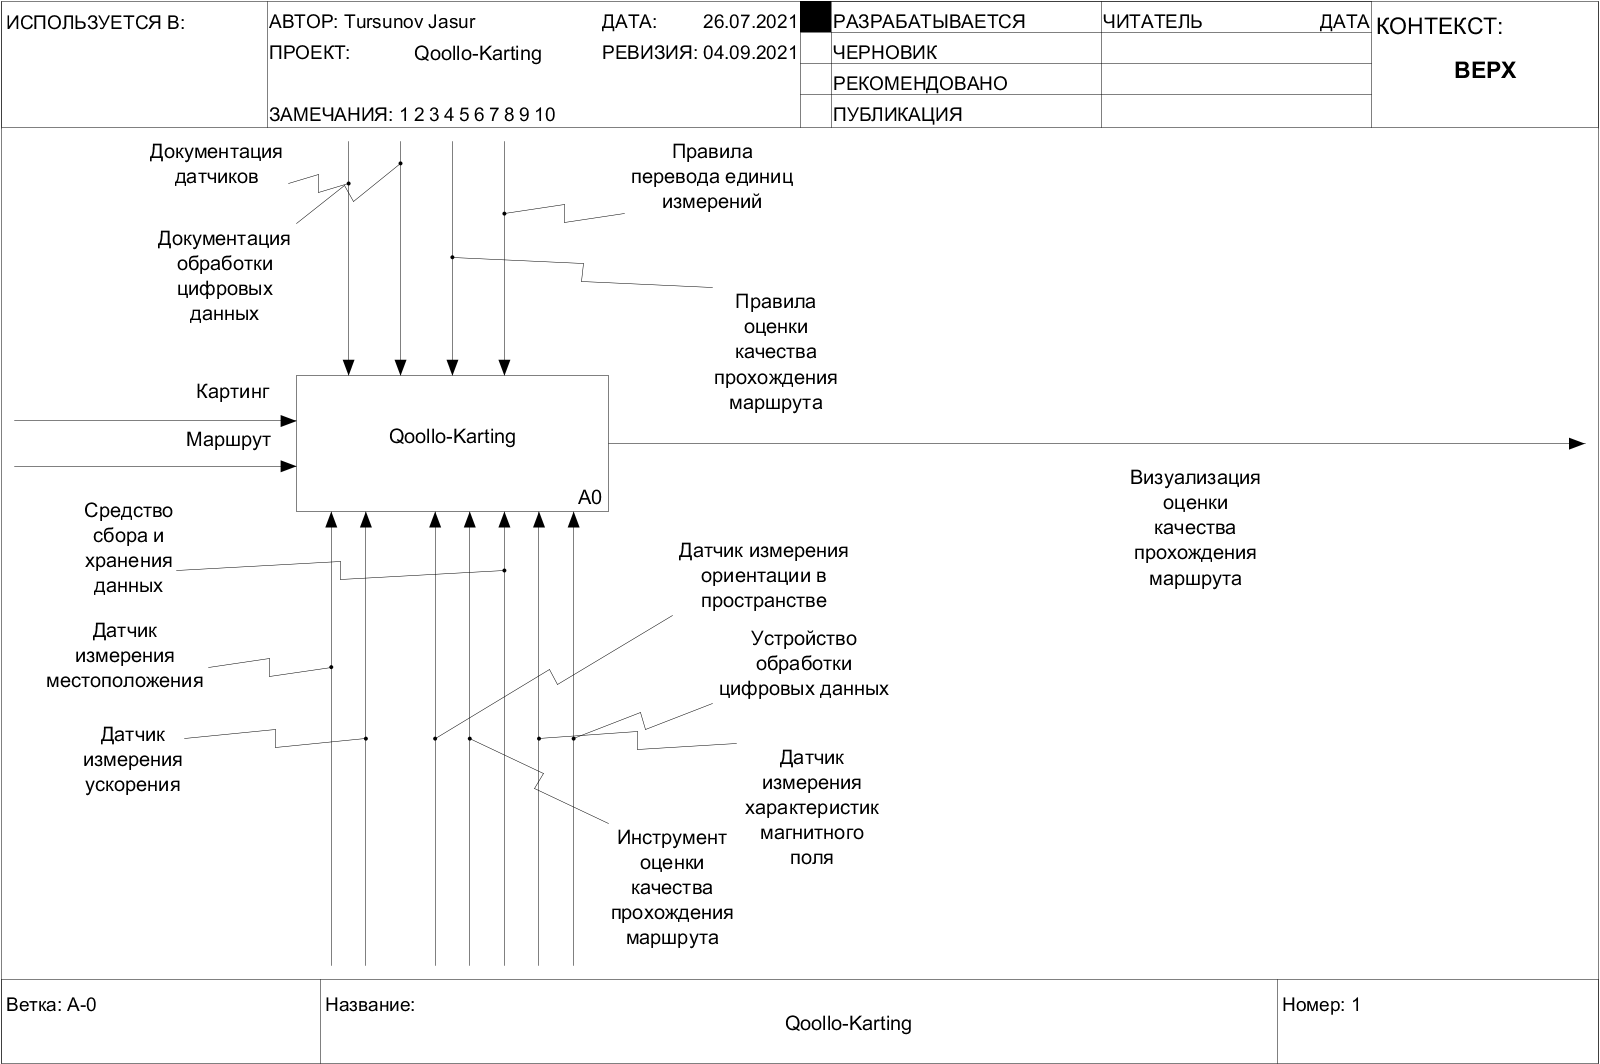
\includegraphics[scale=0.22]{idef0}
		\centering\caption{Декомпозиция функциональной модели IDEF0}
	\end{figure}
	\begin{figure}[h!]
		\centering
		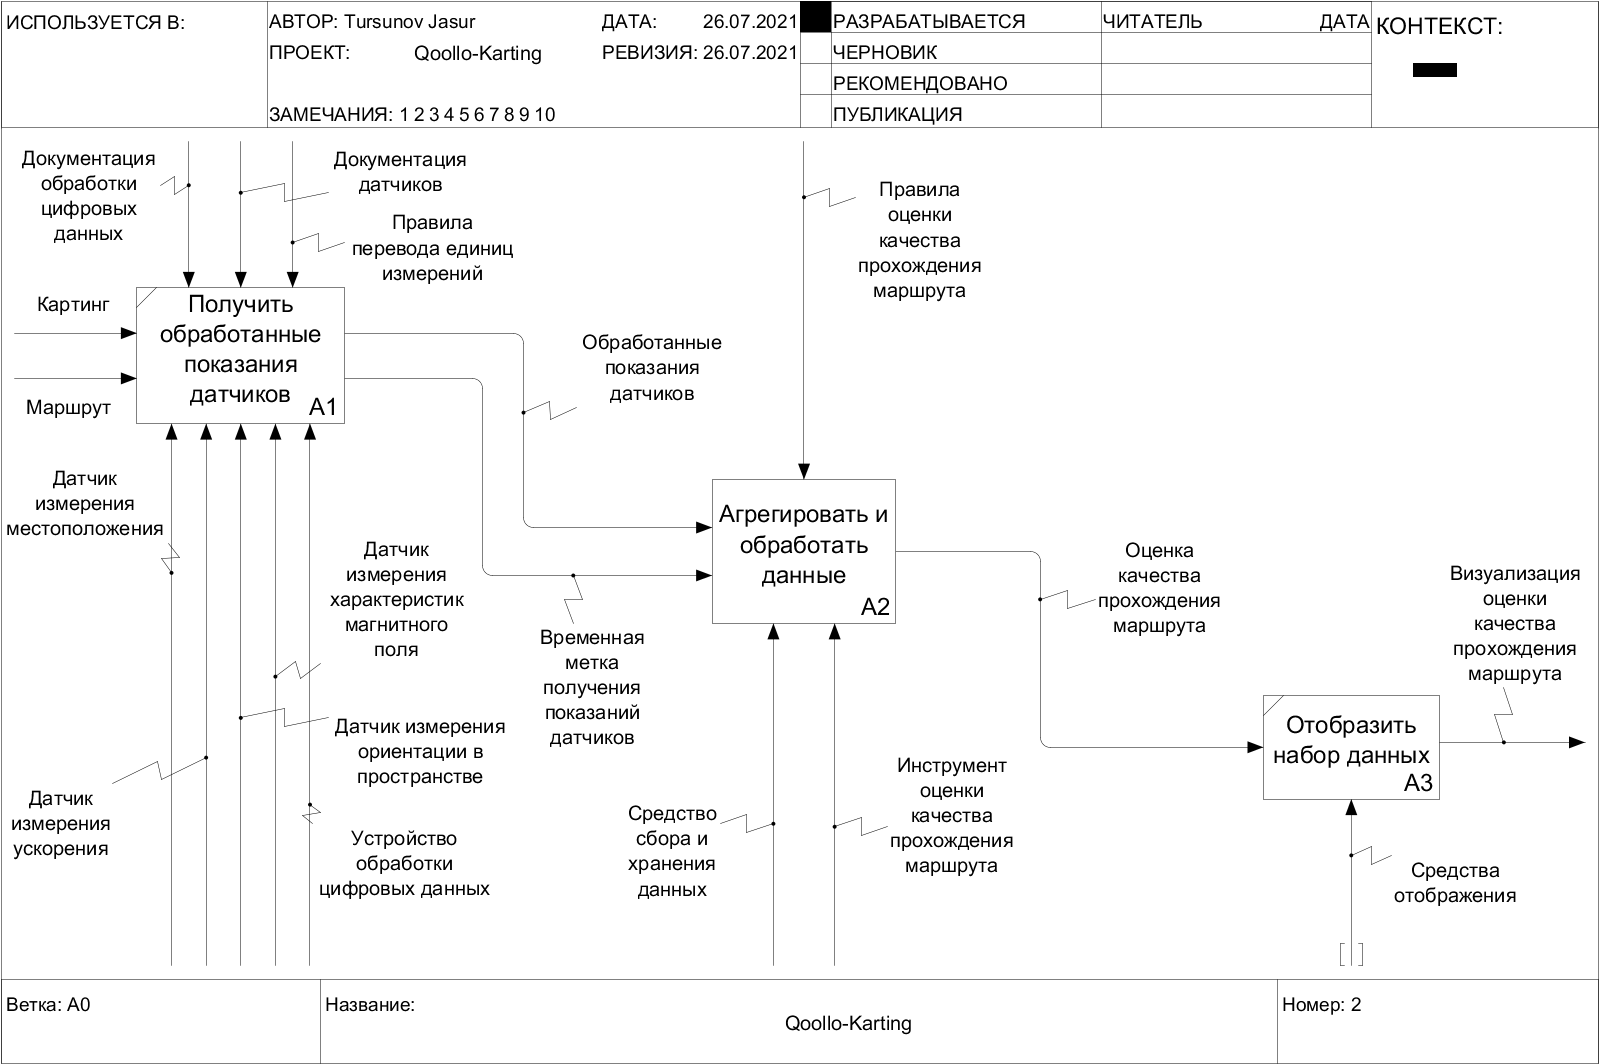
\includegraphics[scale=0.22]{idef1}
		\centering\caption{Декомпозиция функциональной модели IDEF0}
	\end{figure}
	\section{Командная разработка}
	\hspace*{5mm} Во главе ментора и четырех разработчиков была организована командная работа. Для контроля статуса выполнения задач и четкого понимания сроков выполнения поставленных задач перед каждым участником, был использован Redmine. В качестве системы управления версиями в рамках разрабатываемого проекта использовался Git.   
	\section{Архитектура программно-аппаратного комплекса} 
	\hspace*{5mm} В ходе совместной работы, командой была разработана архитектура программно-аппаратного комплекса, которая представлена на рисунке 3. В качестве типа архитектуры предпочтение было отдано микросервисной архитектуре, так как было четко ясно, что программно-аппаратный комплекс будет разбит на небольшие автономные компоненты, изменение которых не будет влиять на работоспособность других частей. Проект имеет архитектуру, с единой точной входа, базой данных, сервисом хранения данных маршрутов, сервисом оценки маршрута, сервисом тайлов. Для взаимодействия компонентов была использована архитектура REST. Выбор стиля взаимодействия основывался на таких качествах как: простота интерфейсов, надежность, масштабируемость, возможность использовать разные языки программирования для разных компонент. В общем случае REST является простым интерфейсом управления информацией без использования каких-то дополнительных внутренних настроек. Каждая единица информации однозначно определяется глобальным идентификатором, таким как URL. URL - это адрес, который выдан уникальному ресурсу в интернете. Каждая URL в свою очередь имеет строго заданный формат[1]. 
	\\ \hspace*{5mm} Управление информацией сервиса – полностью основывается на протоколе передачи данных. Наиболее распространенный протокол - HTTP. Для HTTP действие над данными задается с помощью методов: GET (получить), PUT (добавить, заменить), POST (добавить, изменить, удалить), DELETE (удалить). Таким образом, действия CRUD (Create-Read-Updtae-Delete)[2] могут выполняться как со всеми 4-мя методами, так и только с помощью GET и POST.
	\clearpage
	\newpage
	\begin{figure}[h!]
		\centering
		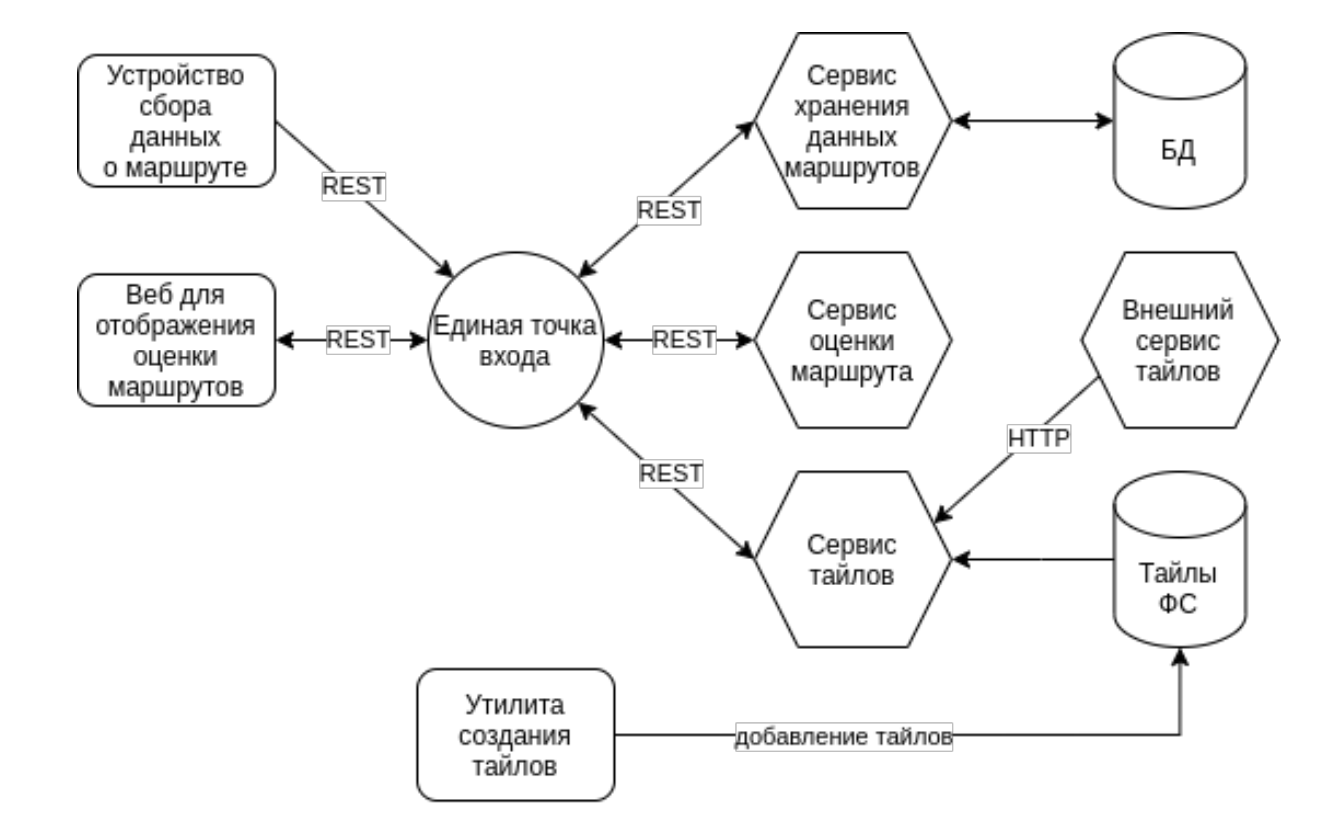
\includegraphics[scale=1]{arch}
		\centering\caption{Архитектура проекта}
	\end{figure}
    Начальная версия сервиса уже была написана ранее. Одной из поставленных задач было разработка и добавление новых функций в уже существующую реализацию. 
	\section{Сервис хранения данных маршрутов}
	\hspace*{5mm} Первая реализация сервиса была написана с использованием микрофреймворка Flask. Исходя из этого новый функционал продолжил использовать этот фреймворк. Flask — микрофреймворк для создания веб-приложений на языке программирования Python, использующий набор инструментов Werkzeug, а также шаблонизатор Jinja2. Перед тем как начать создавать новый функционал, необходимо было разобраться в уже существующем коде, чтобы не разрушать уже проделанную работу. Для разрабатываемого сервиса была написана документация, с подробным описанием всех POST и GET запросов. Ниже показаны все запросы обрабатываемые сервисом. Последние 4 запроса были реализованы в новой версии проекта.
	\begin{enumerate}
		\item создать маршрут;
		\item добавить координаты маршрута;
		\item получить список маршрутов;
		\item добавить показания датчиков;
		\item получить список показаний датчиков;
		\item список координат маршрута.
	\end{enumerate}
	На рисунке 4 показана функциональная модель IDEF0 второго уровня, в которой подробно описана схема работы сервиса хранения данных маршрута. 
	\begin{figure}[h!]
		\centering
		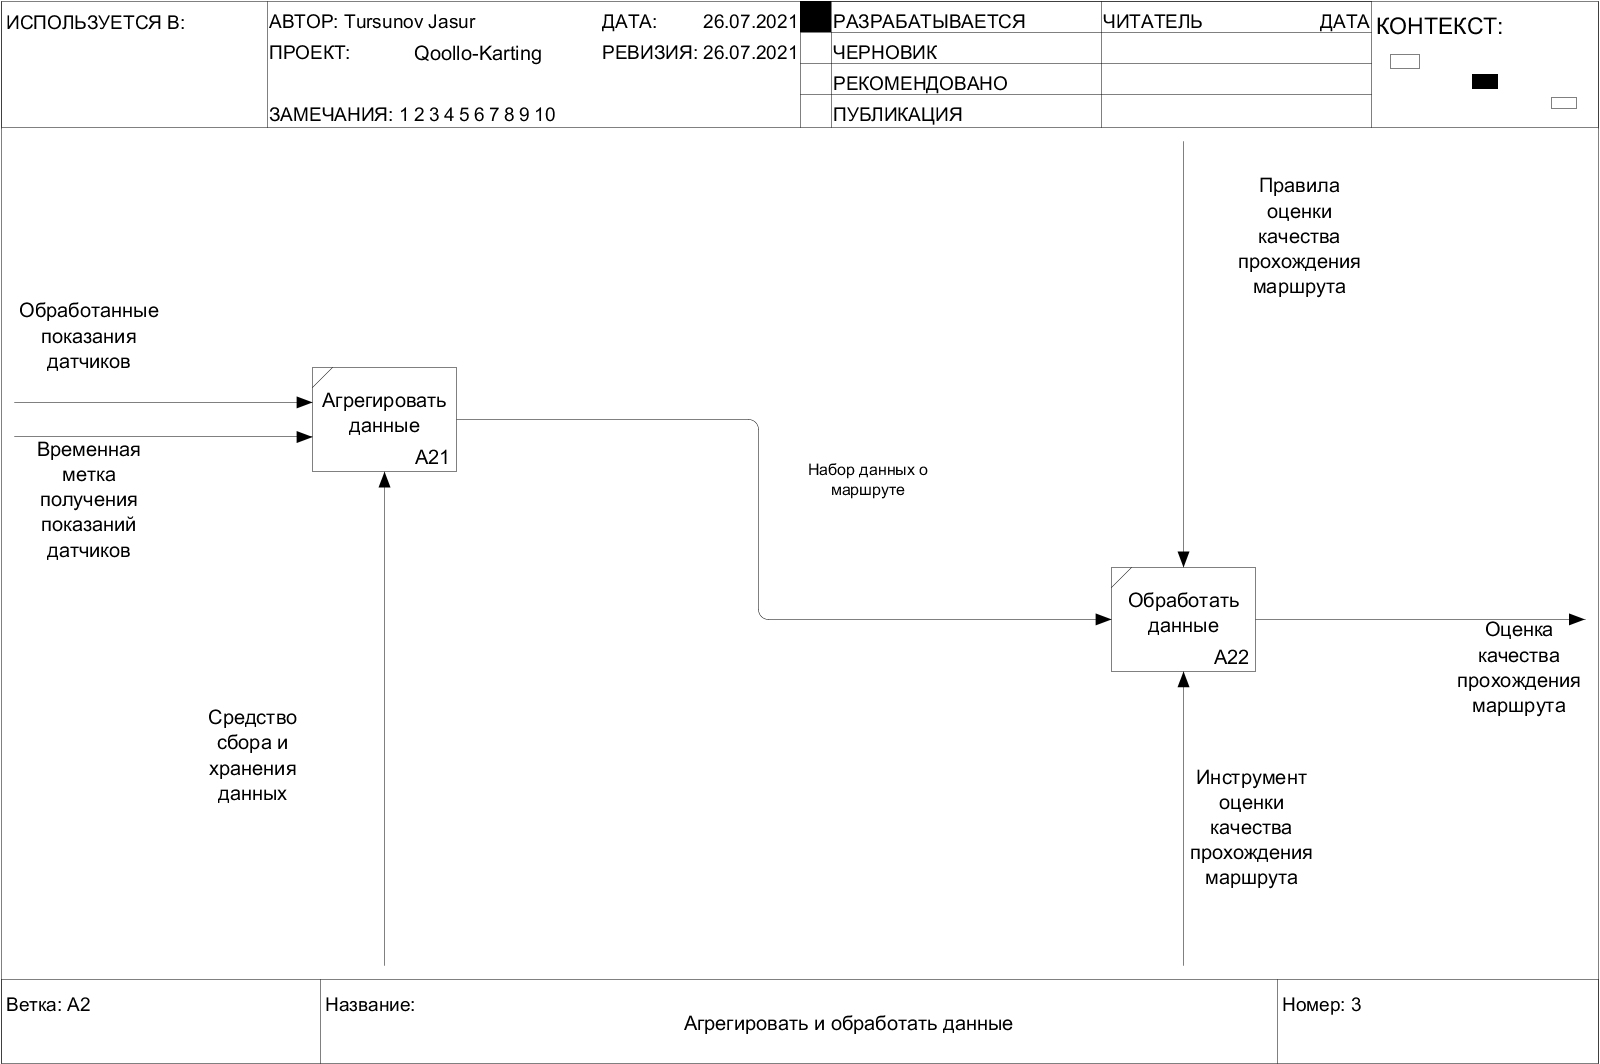
\includegraphics[scale=0.25]{idef2}
		\centering\caption{Декомпозиция функциональной модели IDEF0}
	\end{figure}  
	\section{База данных}
	\hspace*{5mm} Не смотря на то, что существует разные типы баз данных, в данной работе была выбрана реляционная модель. Эта модель была выбрана из вида наших данных к которым применимы следующие достоинства:
	\begin{enumerate}
		\item доступность для понимания пользователем. Единственной используемой информационной конструкцией является "таблица";
		\item полная независимость данных. Изменения в прикладной программе при изменении реляционной БД минимальны;
		\item для организации запросов и написания прикладного ПО нет необходимости знать конкретную организацию БД во внешней памяти. 
	\end{enumerate}
	\hspace*{5mm} Для упрощения процесса сохранения объектов в реляционную базу данных и их извлечения была использована ORM. ORM - это технология программирования, которая позволяет преобразовывать несовместимые типы моделей в ООП, в частности, между хранилищем данных и объектами программирования. ORM сама заботится о преобразовании данных между двумя несовместимыми состояниями. Большинство ORM-инструментов в значительной мере полагаются на метаданные базы данных и объектов, так что объектам ничего не нужно знать о структуре базы данных, а базе данных — ничего о том, как данные организованы в приложении. ORM обеспечивает полное разделение задач в хорошо спроектированных приложениях, при котором и база данных, и приложение могут работать с данными каждый в своей исходной форме. Использование ORM не ограничивает выбор БД. Можно в любой момент поменять на подходящую БД.
	\\ \hspace*{5mm} На рисунке 5 показана ER-диаграмма, описывающая концептуальные схемы разрабатываемой предметной области. База данных состоит из 3 таблиц: track, coordinate, sensor.
	\\ \hspace*{5mm} В таблице track хранится уникальная номер о маршруте. Каждый маршрута имеет неограниченное число значений датчиков, в следствие чего, создана таблица coordinate, которая направлена на хранение информации о местоположение карта. Эта модель связана с таблицой sensor, в которой хранится данные с акселерометра, магнитометра, гироскопа.
	\begin{figure}[h!]
		\centering
		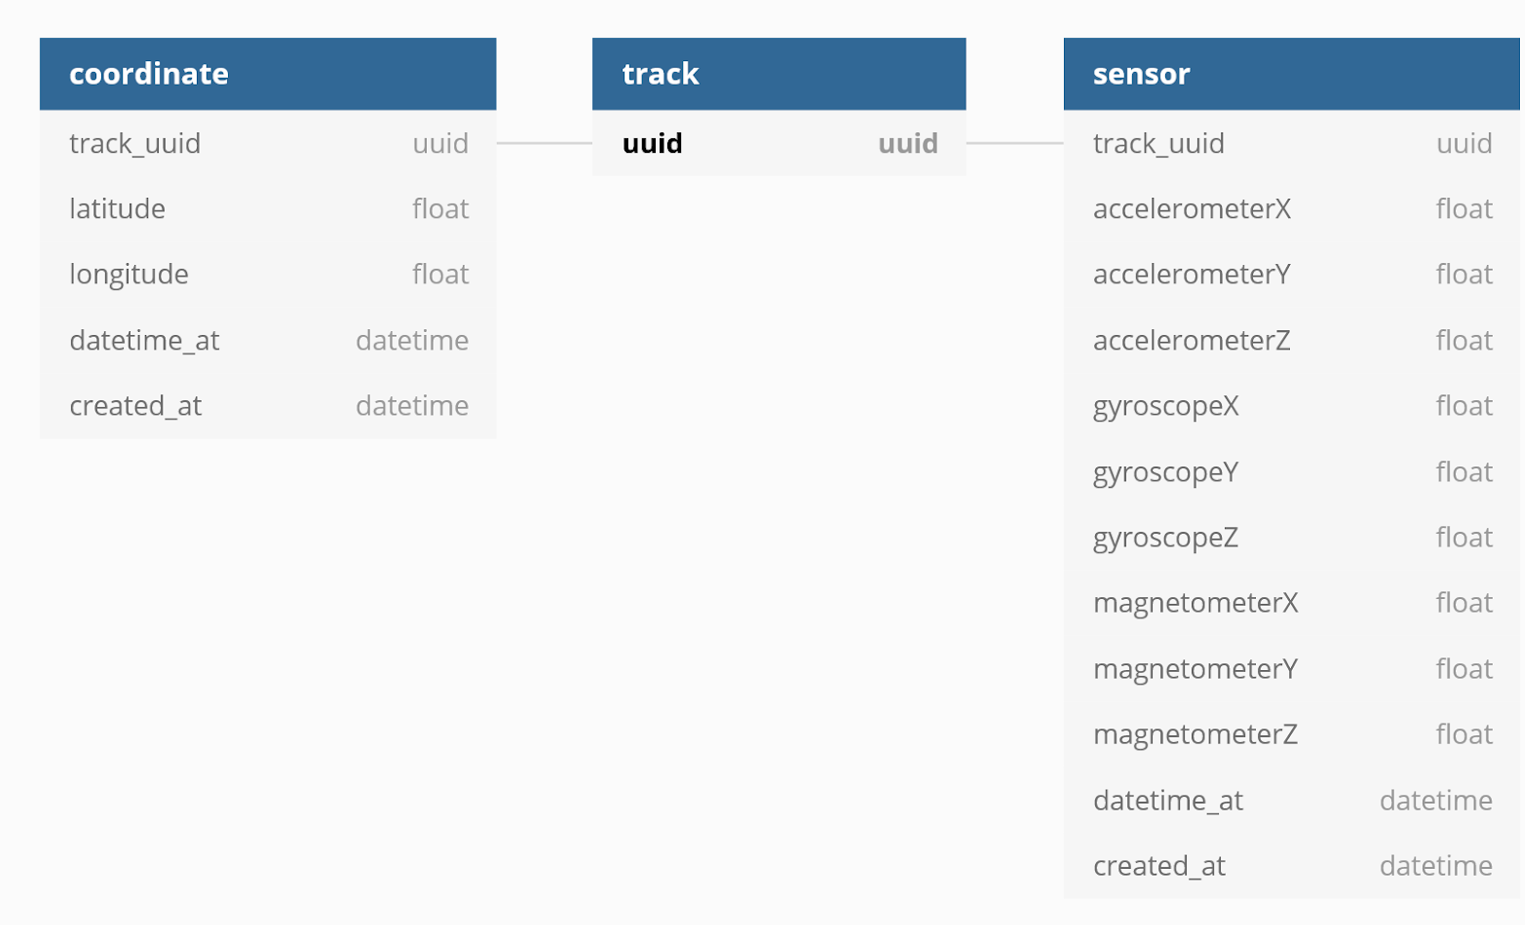
\includegraphics[scale=0.8]{er-diagram}
		\centering\caption{ER-модель структуры БД}
	\end{figure}
	 \section{Используемые инструменты и технологии веб-приложения}
	\hspace*{5mm} Для облегчения разработки веб-приложения нужно использовать фреймворки, которые являются набором шаблонов или заготовок, облегчающий разработку и объединение разных модулей программного проекта.   
	\\ \hspace*{5mm} Для разработки API был использован универсальный микрофреймворк с открытым исходным кодом Flask[3]. Для работы с базой данных использовалась ORM SQLArchemy, в которой модель данных описывается классами Python, и по ней генерируется схема базы данных. В качестве среды разработки выбран редактор PyCharm[4]. 
	\\ \hspace*{5mm} Для удобства проверки запросов с клиента на сервер и получения обратного ответа было использовано приложение Postman[5].
	\\ \hspace*{5mm} Для тестирования производительности, сбора показателей и определения производительности и времени отклика программно-технической системы был использован инструмент Яндекс.Танк[6]. 
	\\ \hspace*{5mm} В качестве инструмента для хранения и управления репозиториями Git был выбран GitLab[7]. GitLab дает возможность выполнять совместную разработку силами нескольких программистов, применять обновления кода и откатывать изменения, если это необходимо.
	\\ \hspace*{5mm} Для управления задачами проектами, учёта временных затрат, отслеживания статуса выполнения задачи было решено использовать веб-приложение Qoollo Redmine. 
	\section{Системные характеристики}
	Характеристики компьютера на котором проводился эксперимент:
	\begin{enumerate}
		\item операционная система - Windows 10(версия 10.0.19043);
		\item процессор - Intel(R) Core(TM) i7-10510U CPU @1.80GHz 2.30GHz, количество ядер - 4, количество логических процессов - 8;
		\item объем оперативной памяти - 16 ГБ, тип оперативной памяти - DDR4, скорость оперативной памяти - 2133 МГц, количество планок оперативной памяти - 2, режим работы оперативной памяти - двухканальный;
		\item скорость записи и чтения жесткого диска - 193 MB/s.
	\end{enumerate} 
	
	\section{Модульное тестирование}
	\hspace*{5mm} В рамках данного проекта были написаны 15 модульных тестов, направленные на проверку корректного добавления, получения данных из БД. Тестирование было написано с помощью фреймворка unittest, входящий в стандартную библиотеку языка Python[8]. На рисунке 6 показаны результаты тестирования.
		\begin{figure}[h!]
		\centering
		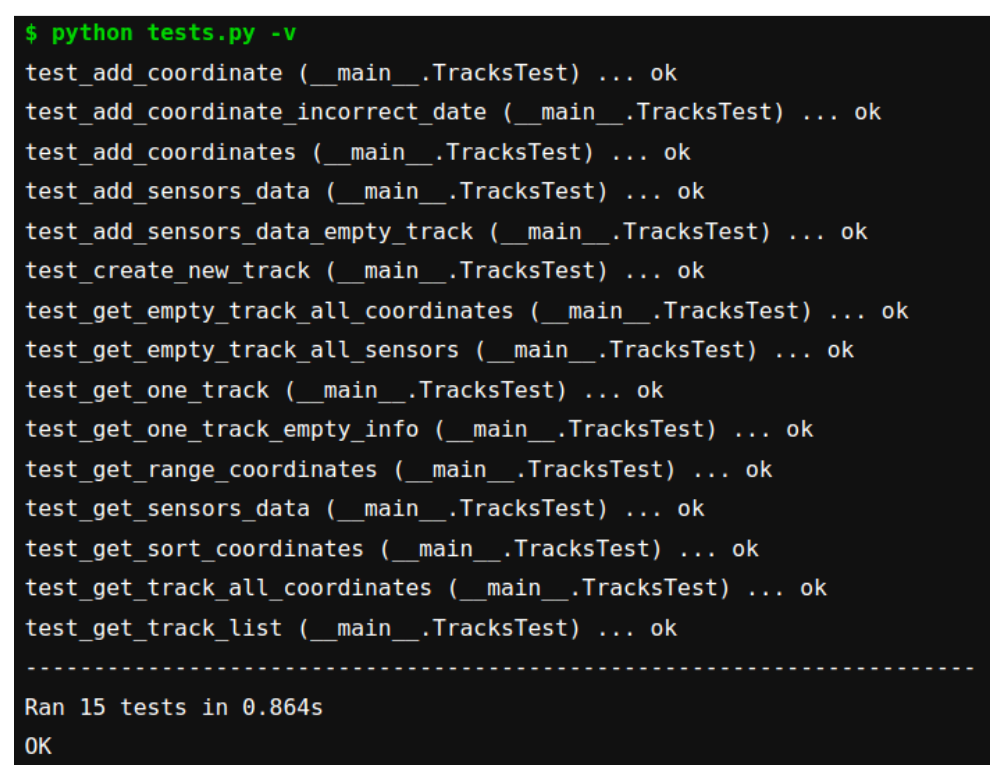
\includegraphics[scale=1.4]{tests}
		\centering\caption{Результаты тестиривания}
	\end{figure}
	\section{Нагрузочное тестирование}
	\hspace*{5mm} Для анализа работоспособности сервиса было проведено нагрузочное тестирование с помощью инструмента Yandex-Tank. Были проведены следующие тесты:
	\begin{enumerate}
		\item для определения максимального количества запросов, которые может обработать сервис, был реализован тест с ступенчатым увеличением запросов, где в каждом запросе добавлялось по одной координате. Промежуток количества запросов был от 0 до 180, с шагом 10 и по 30 секунд для каждого запроса. На рисунке 7 показан полученный результат. Можно заметить, что сервис может отработать без ошибок до 140 запросов в секунду. Для увеличения числа запросов можно оптимизировать запросы к БД или проставить индексы при обращении к базе данных;
		\begin{figure}[h!]
			\centering
			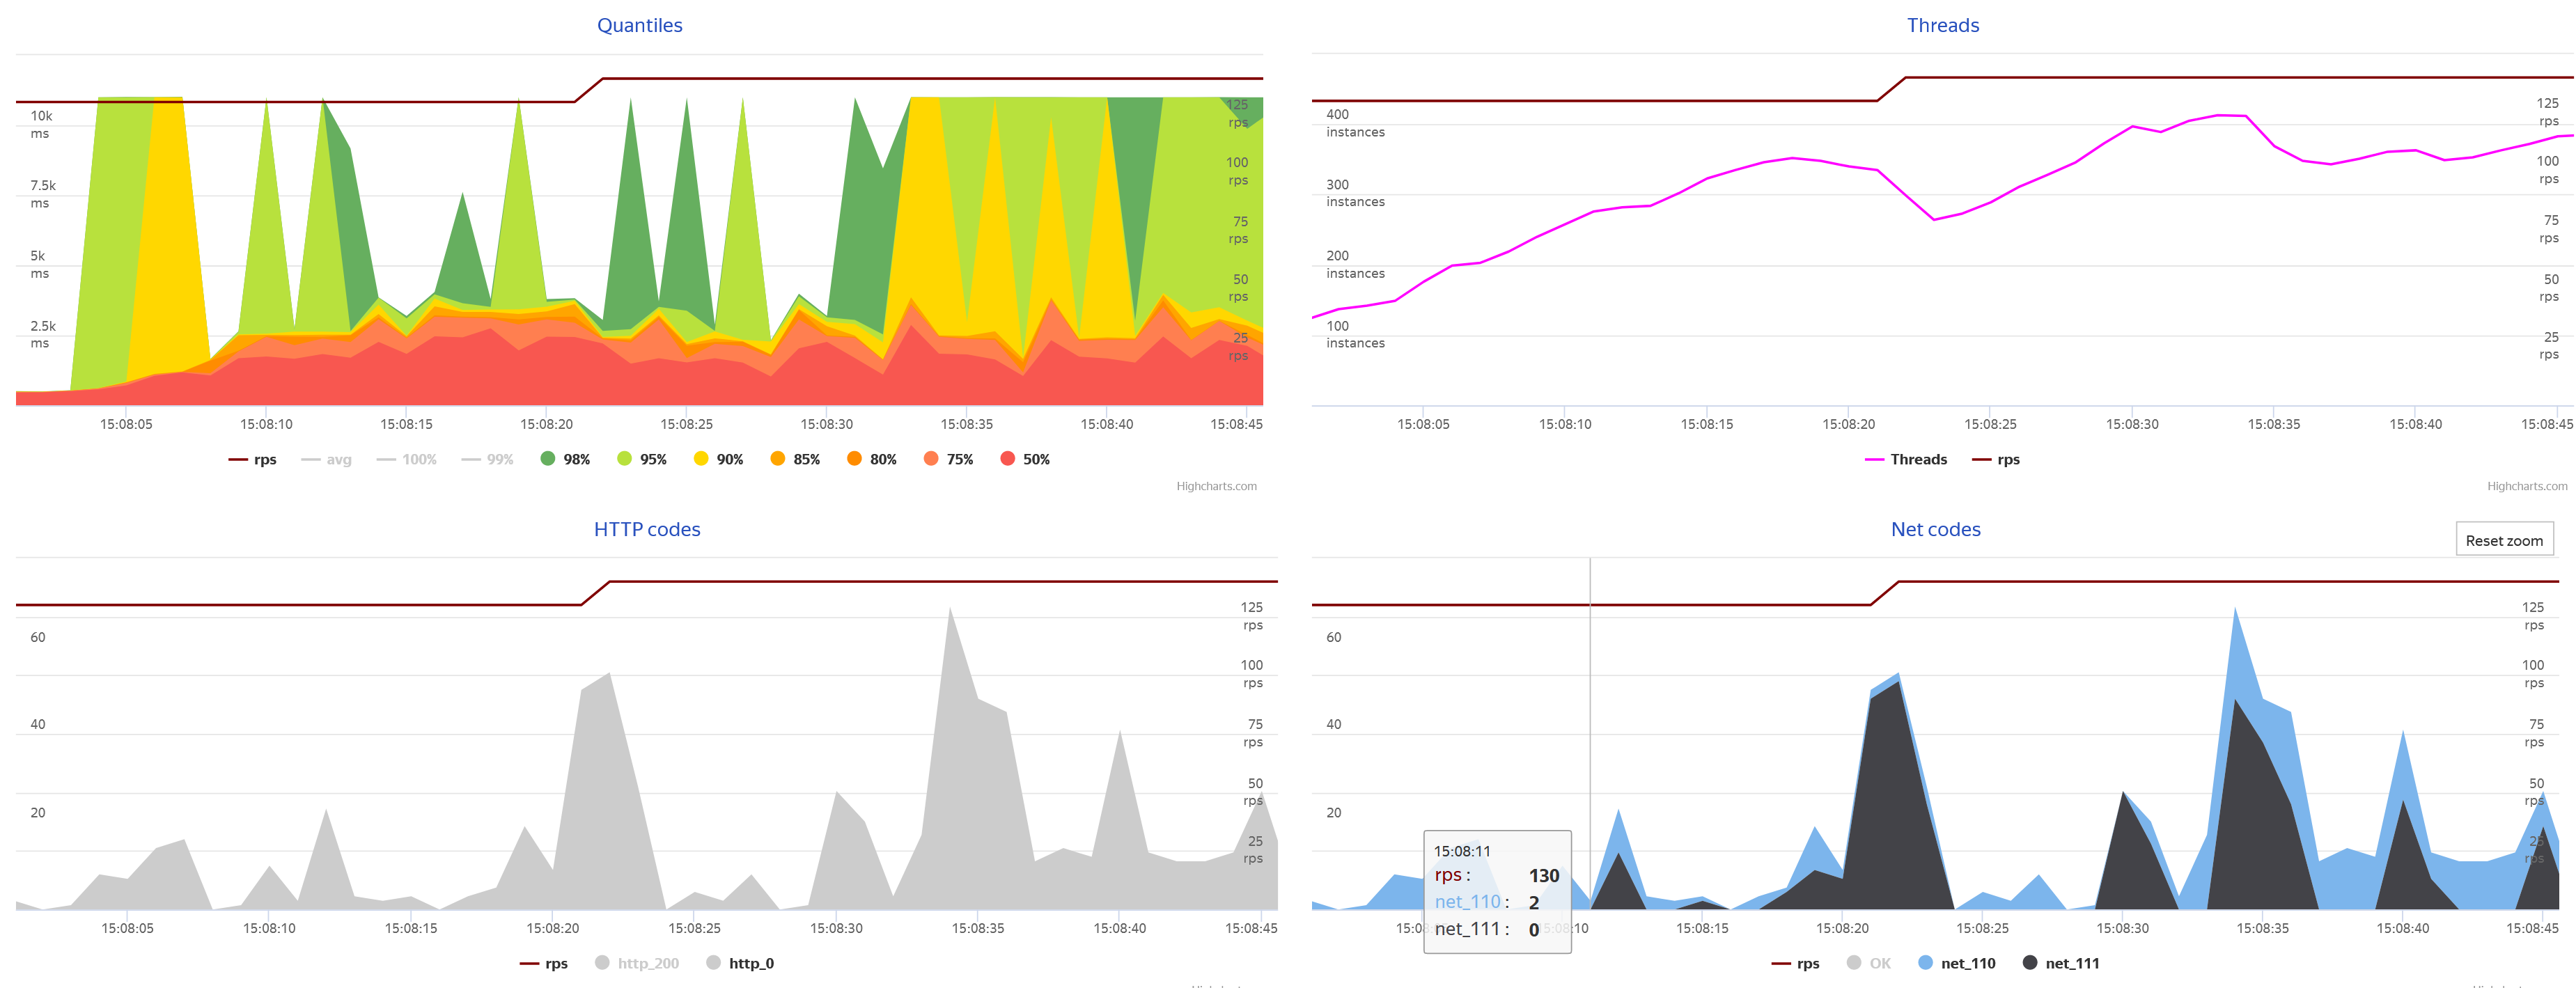
\includegraphics[scale=0.4]{max}
			\centering\caption{Результаты измерения пиковой нагрузки}
		\end{figure}
		\item чтобы определить сможет ли сервис обработать до 140 запросов, если добавление координат за каждый запрос будет не по одной, а по несколько - 5. Все параметры теста идентичны с предыдущим тестом. На рисунке 8 представлены результаты моделирования. Как видно из рисунка работоспособность сервиса не изменились даже при добавлении 5 координат за раз;
		\begin{figure}[h!]
			\centering
			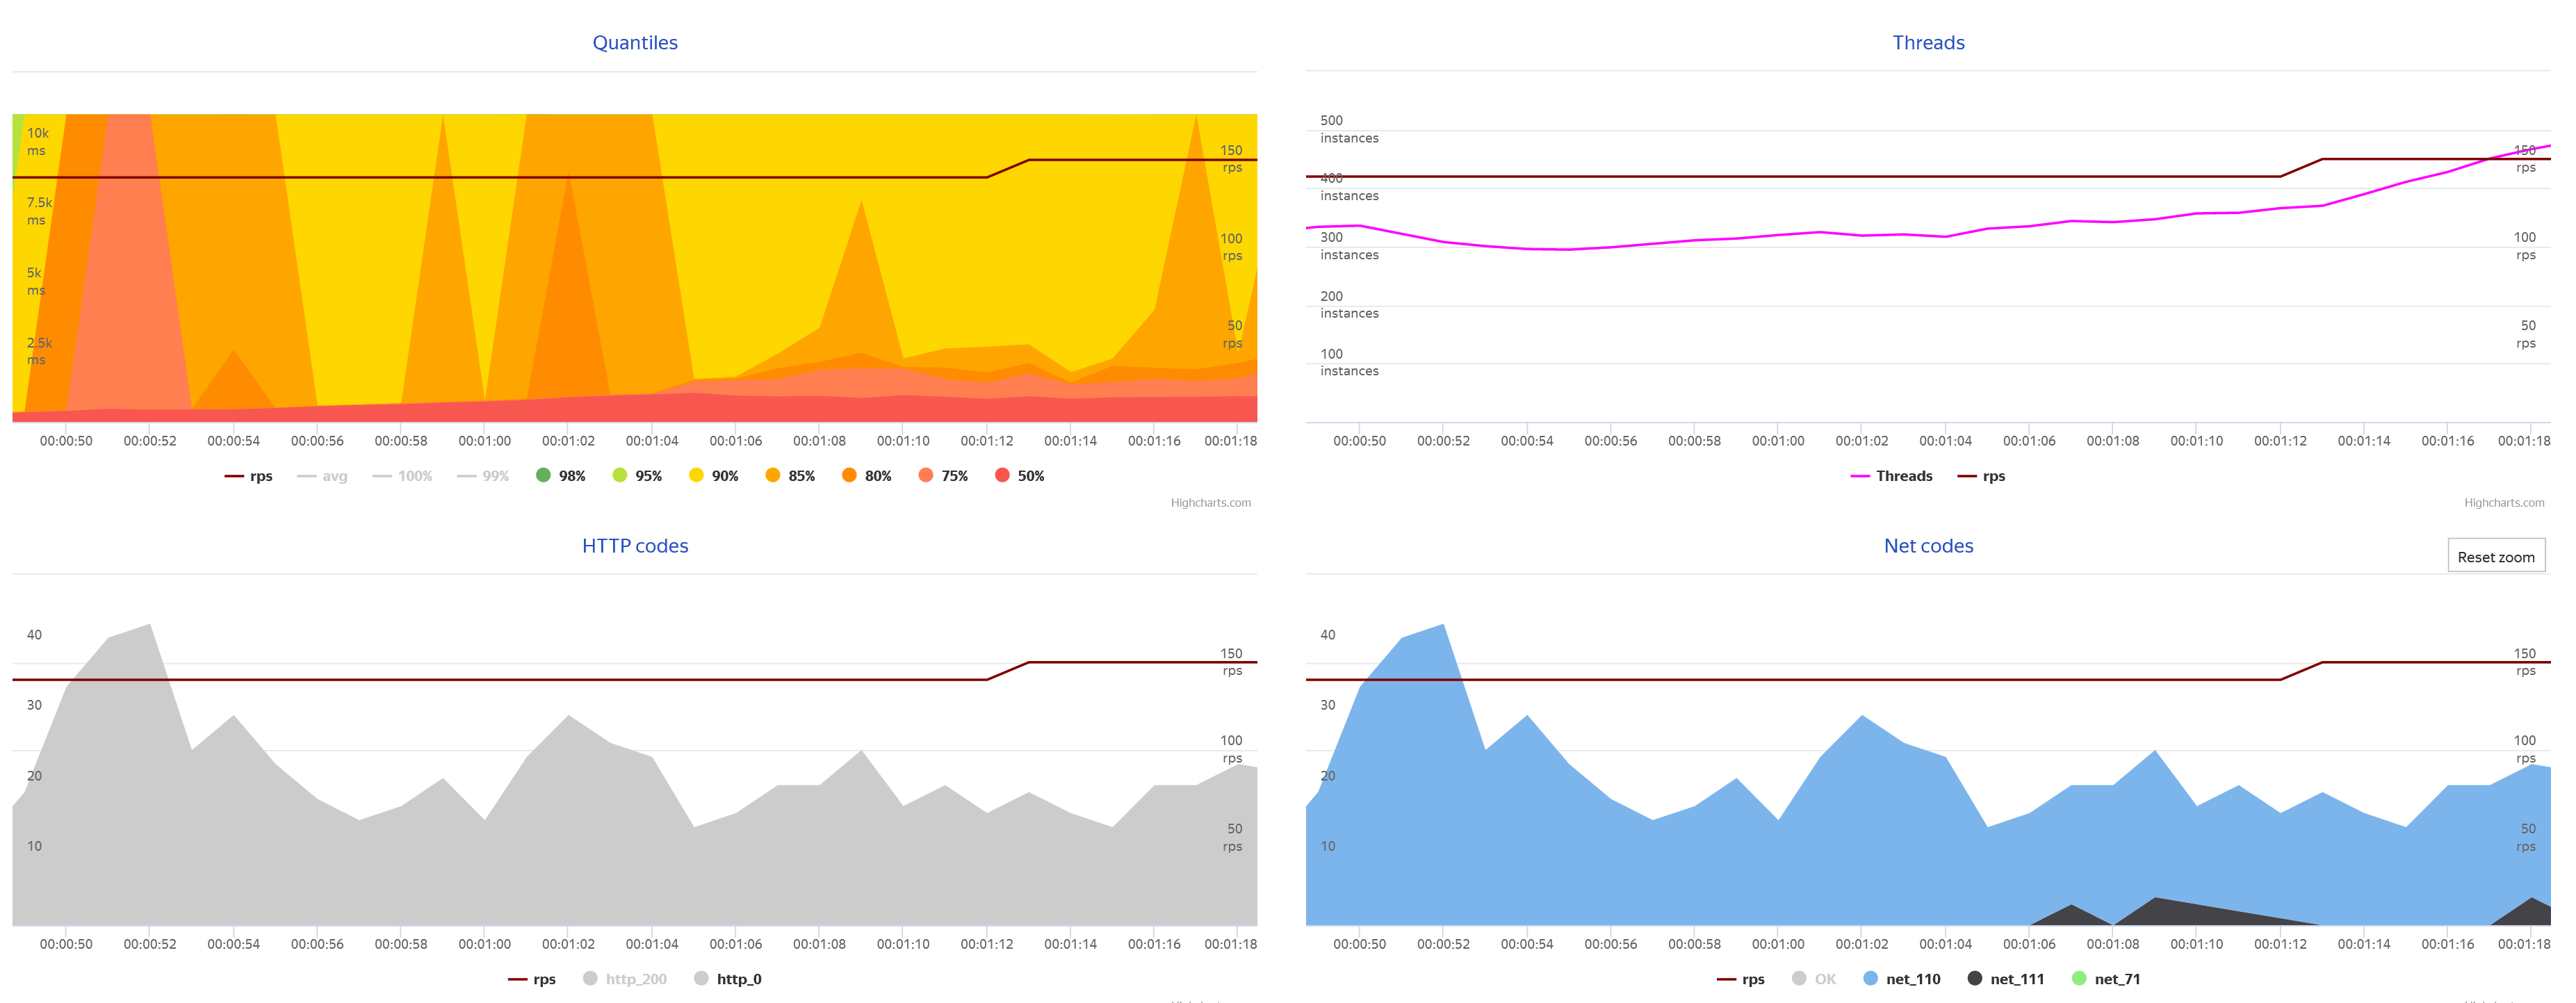
\includegraphics[scale=0.4]{5}
			\centering\caption{Результаты измерения пиковой нагрузки при добавлении 5 координат за раз}
		\end{figure}
		\item восстановление сервиса после кратковременной пиковой нагрузки добавления координат. Данный тест был направлен на то, чтобы узнать сколько времени понадобится сервису чтобы восстановится после кратковременной нагрузки. В ходе тестирования сначала сервис нагружался в пол нагрузки, затем вдвое больше, а затем снова в пол оборота. На рисунке 9 показано, сервис не смог восстановится в течение 30 секунд после пиковой нагрузки. А вот на рисунке 10 при таких же условиях видно, что 60 достаточно чтобы сервич смог нормально заработать поле перегрузки;
		\begin{figure}[h!]
			\centering
			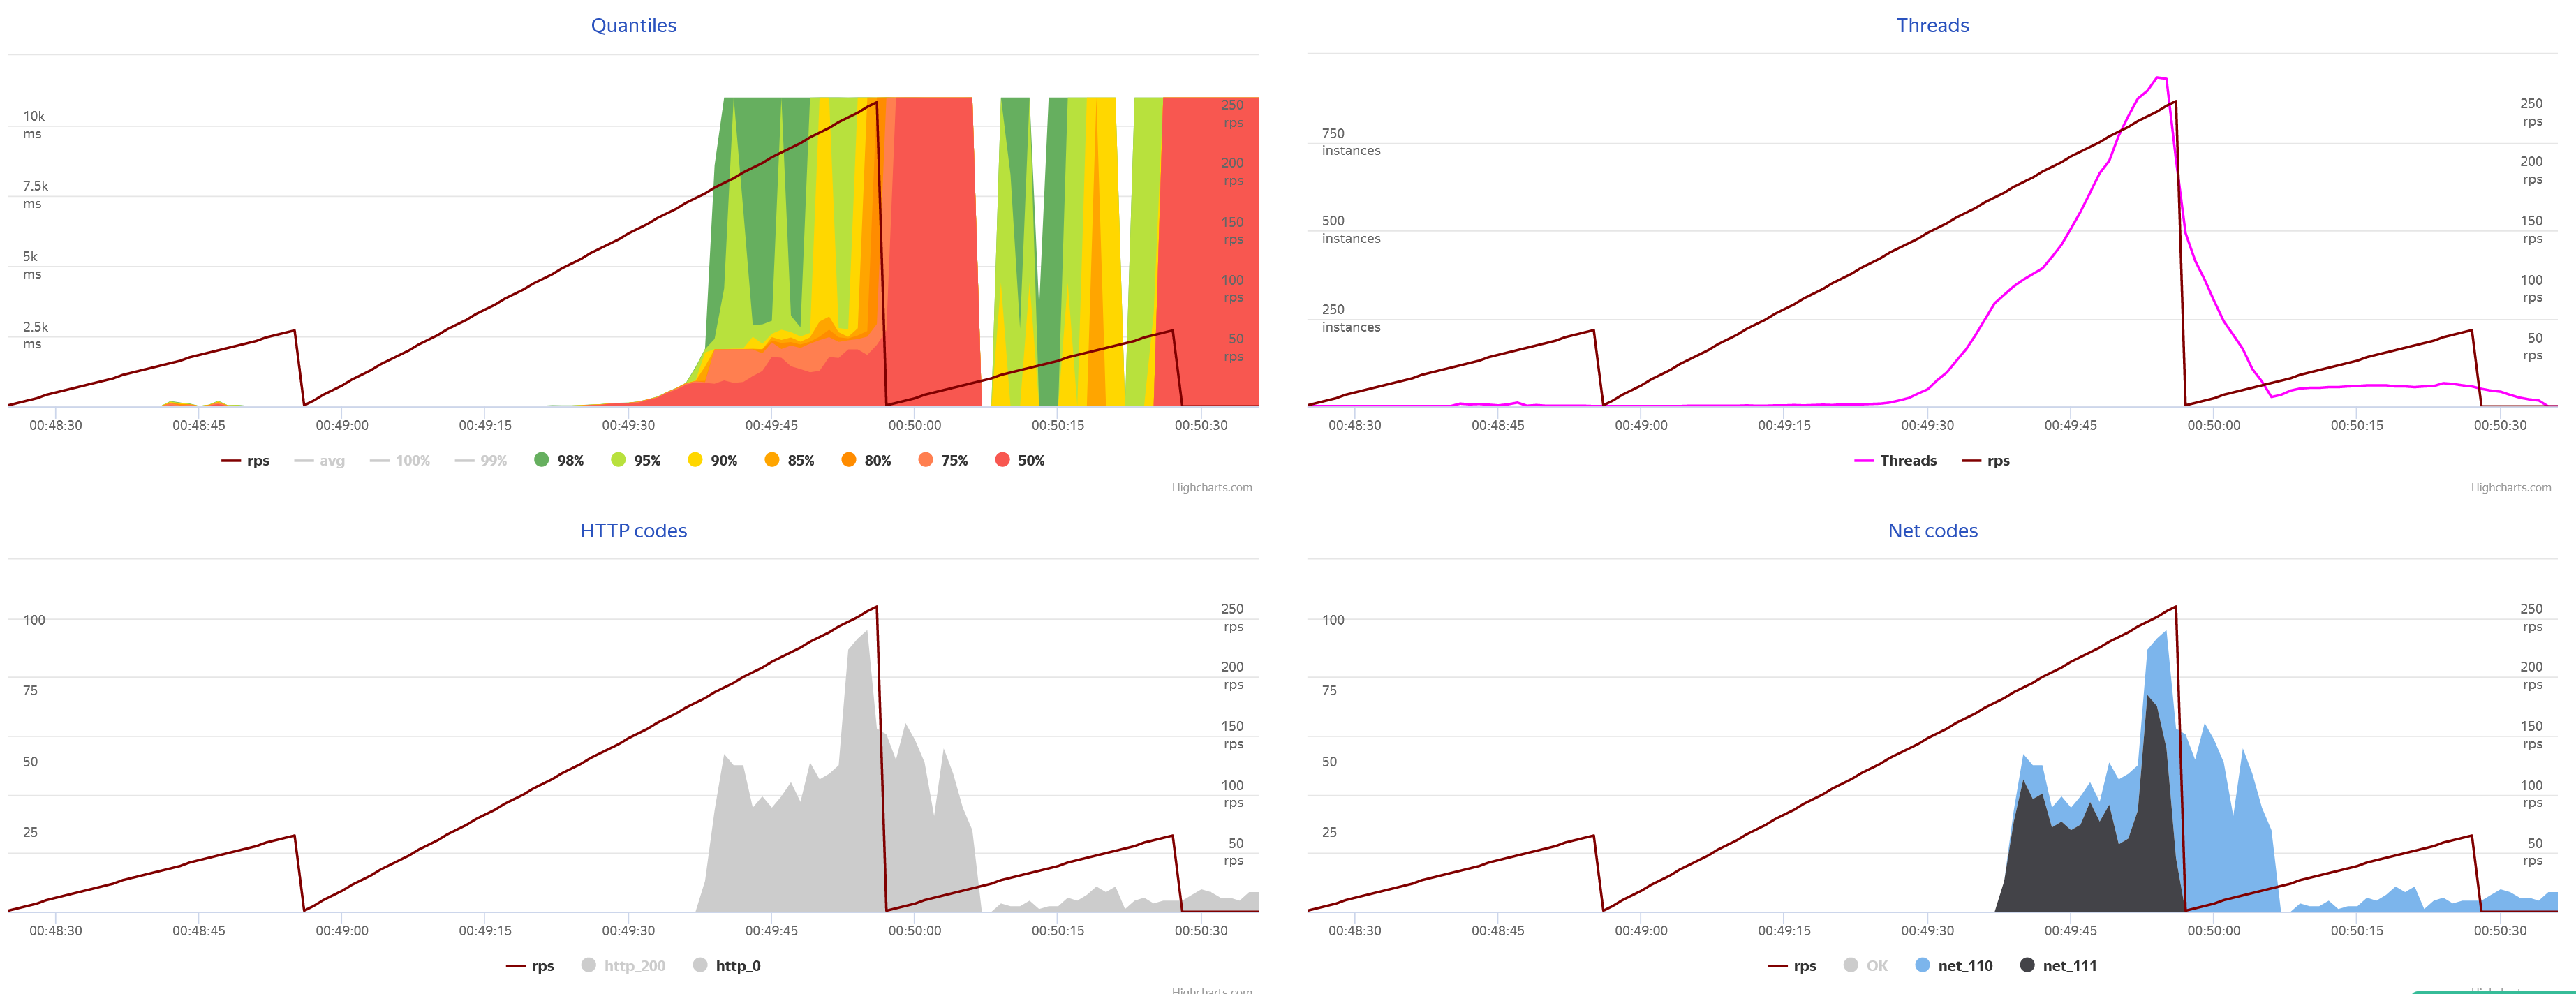
\includegraphics[scale=0.4]{30s}
			\centering\caption{Результаты восстановления сервиса после пиковой нагрузки в течение 30 секунд}
		\end{figure}
		\begin{figure}[h!]
			\centering
			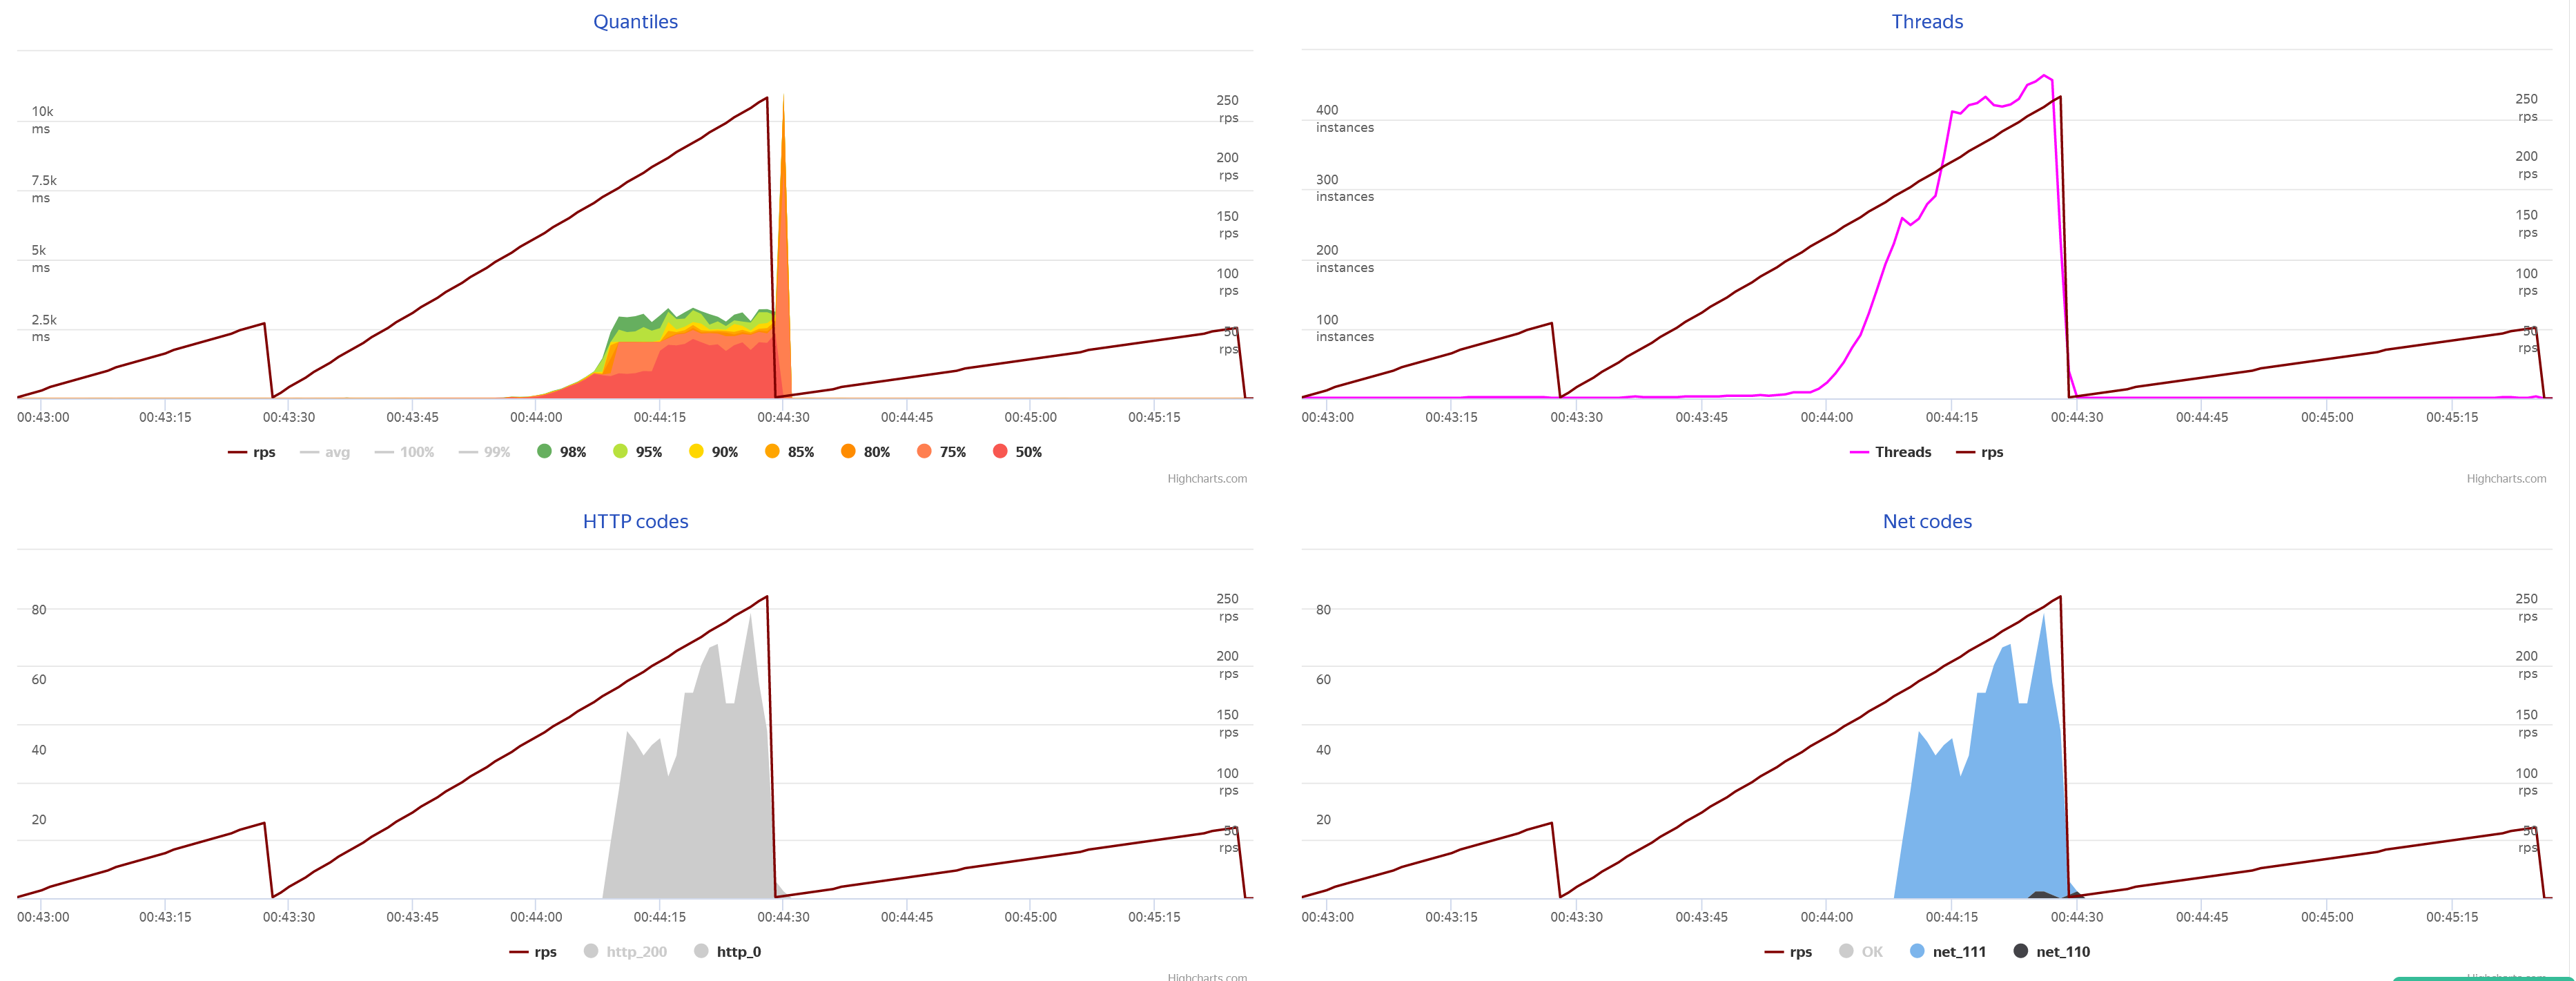
\includegraphics[scale=0.4]{60s}
			\centering\caption{Результаты восстановления сервиса после пиковой нагрузки в течение 60 секунд}
		\end{figure}
		\item чтобы узнать как будет вести себя сервис в течение долгого промежутка времени был проведен тест в котором, добавление координат происходило с постоянной нормальной нагрузкой в течение 60 минут. На рисунке 11 представлены полученные результаты. Можно сделать вывод, что сервис успешно обработал только 69\% всех запросов;
		\clearpage
		\newpage
		\begin{figure}[h!]
			\centering
			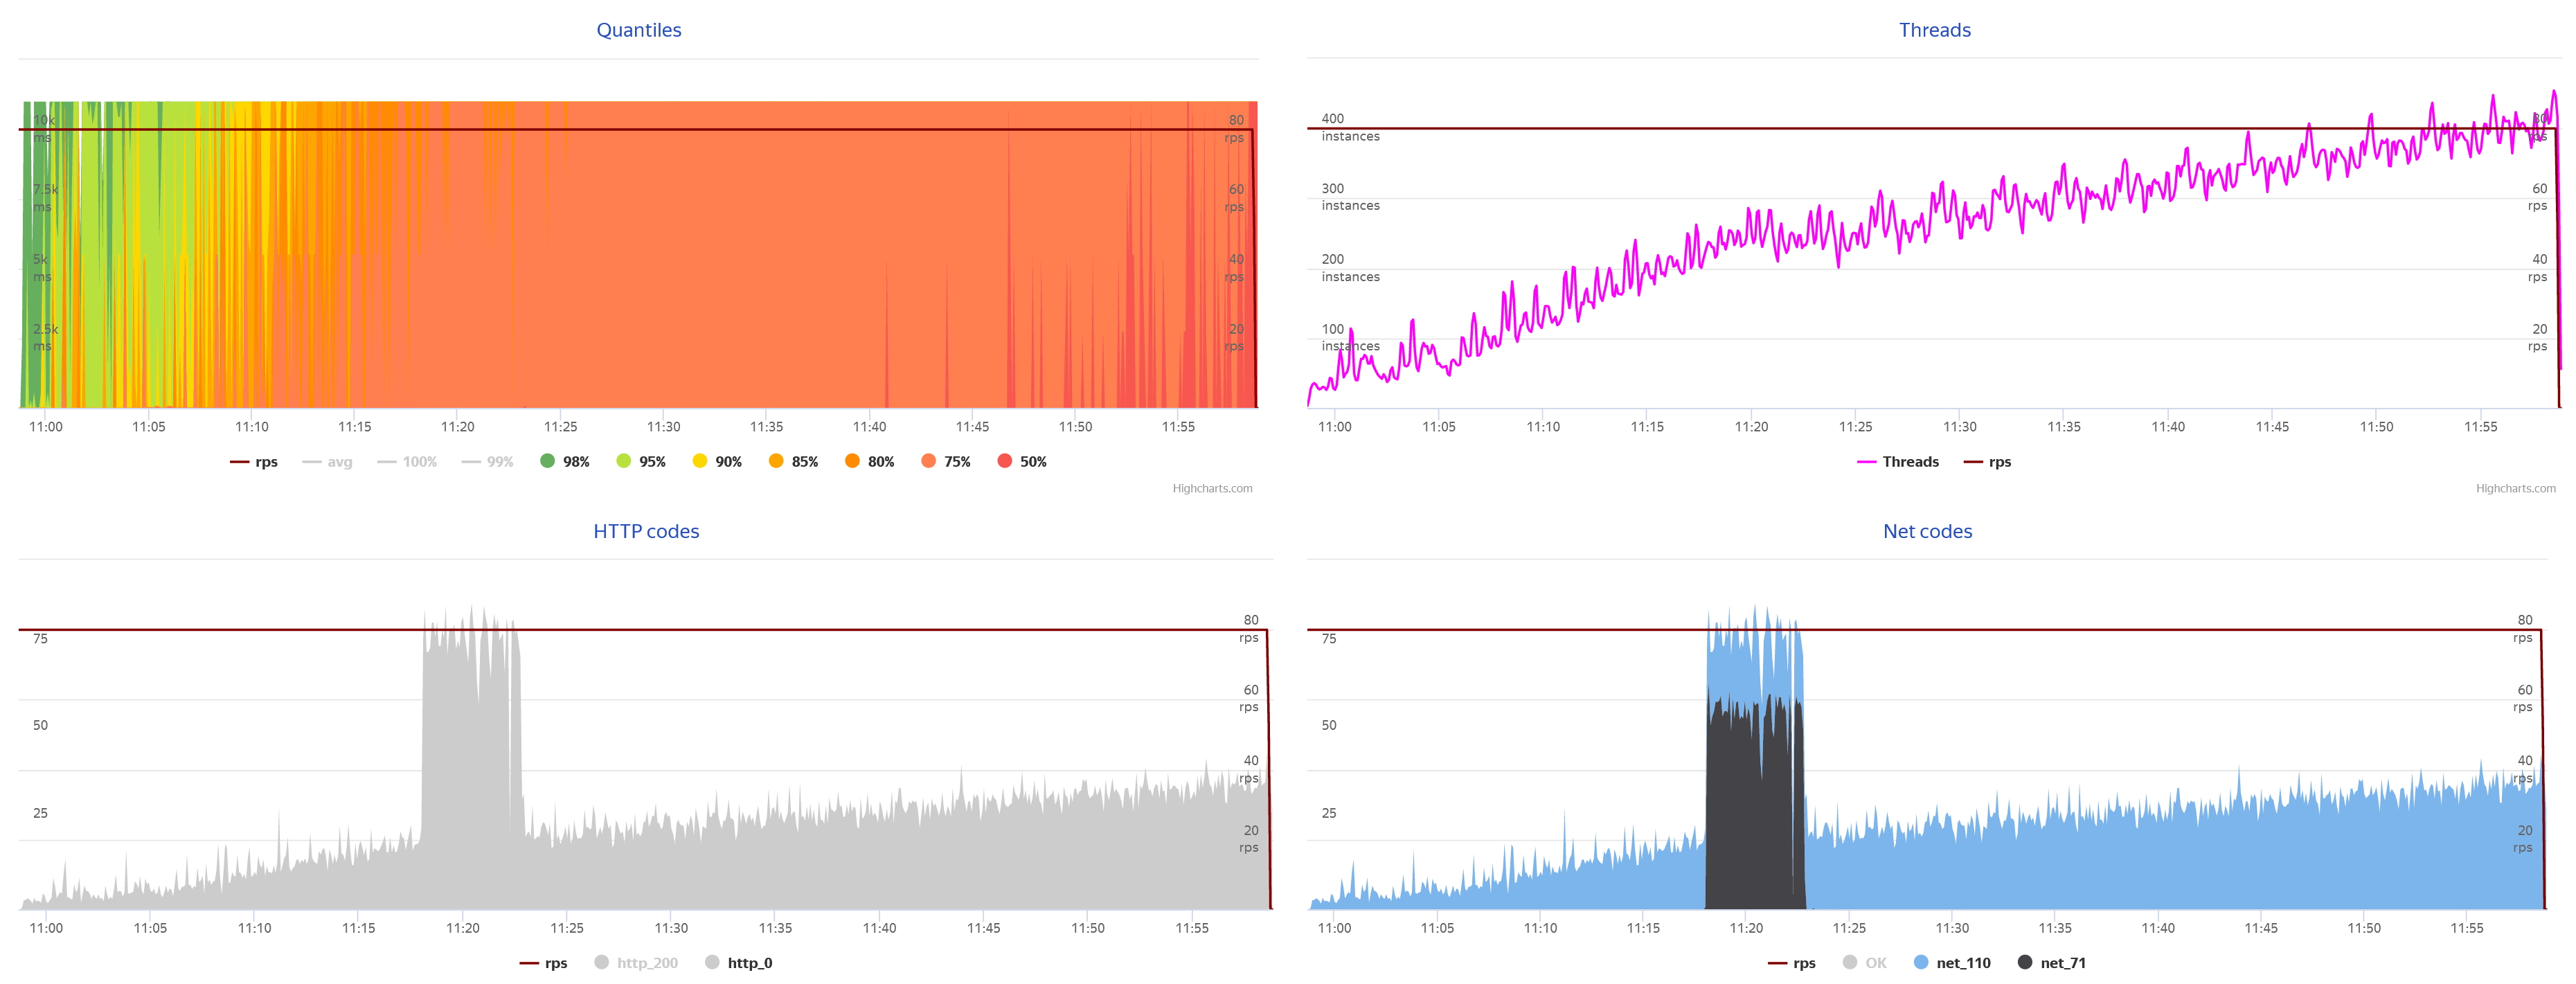
\includegraphics[scale=0.4]{60min}
			\centering\caption{Результаты тестирования в течении 60 минут}
		\end{figure}
	\end{enumerate}
	\clearpage
	\newpage
	\section*{Заключение}
	\addcontentsline{toc}{section}{Заключение}
	\hspace*{5mm}В рамках практики был реализован программно-аппаратный комплекс для оценки качества прохождения маршрутов. С помощью разработанной программы можно получить подробный анализ пройденного маршрута пилотом. В рамках текущего проекта были решены все ранее поставленные индивидуальные задачи: 
	 \begin{enumerate}
		\item умение работать в команде;
		\item разбор уже существовашей реализации сервиса и используемых в ней технологиях;
		\item написание документации к новым функциям для API;
		\item добавление новых функций в API;
		\item проведение модульного тестирования;
		\item проведение нагрузочного тестирования и анализ полученных результатов.
	\end{enumerate}
	\hspace*{5mm}Целью каждого программного обеспечения является уменьшение влияние человеского фактора в разных аспектах, тем самым внедряя машинное обучение мы получаем человеконезависимый продукт. Этот программный комплекс не исключение. Развивая этот проект можно находить оптимальный маршрут, определять физическое, психологическое состояние пилота на разных этапах маршрута и многое другое. 
	   
%\end{flushleft}

\clearpage
\newpage
\section*{Список литературы}
\addcontentsline{toc}{section}{Список литературы}
[1] \hspace{2mm} Архитектура REST // Habr URL: https://habr.com/ru/post/38730 (дата обращения: 04.07.2021).\vspace{3mm}
\newline [2]\hspace{2mm} CRUD // MaxSite URL: https://maxsite.org/page/restful-crud (дата обращения: 15.07.2021).\vspace{3mm}
\newline [3]\hspace{2mm} Flask // Pallet Projects URL: https://flask.palletsprojects.com/en/2.0.x/ (дата обращения.\vspace{3mm} 
\newline [4]\hspace{2mm} PyCharm // JetBrains URL: https://www.jetbrains.com/ru-ru/pycharm/ (дата обращения: 25.07.2021).\vspace{3mm}
\newline [5]\hspace{2mm} Postman // Postman URL: https://www.postman.com/ (дата обращения: 25.07.2021).\vspace{3mm}
\newline [6]\hspace{2mm} Нагрузочное тестирование // Яндекс Танк URL: https://yandex.ru/dev/tank/ (дата обращения: 20.07.2021).\vspace{3mm}
\newline [7]\hspace{2mm} GitLab URL: https://gitlab.com/ (дата обращения: 15.07.2021).\vspace{3mm}
\newline [8]\hspace{2mm} Python // Python Documentation URL: https://www.python.org/ (дата обращения: 03.07.2021).\vspace{3mm}
%\printbibliography
%\addcontentsline{toc}{section}{Список литературы}

\end{document}